\documentclass[a4paper,10.5pt,uplatex]{jsarticle}  %jsarticleでも良いかも
%--脚注の設定
\usepackage{natbib}
\bibpunct[, ]{(}{)}{;}{and}{}{,} %本文での引用の体裁はここで整えられるみたい
\bibliographystyle{apsr2006-2}   %このagsmは編集済みなので注意。ジャーナルが太字にならないようにしてる。ブログ参照。
\usepackage{amsmath}
%--余白の設定
\usepackage[truedimen,margin=20truemm]{geometry}
%--図の設定
\usepackage[dvipdfmx]{graphicx,xcolor} % PDFの利用もOKに
\graphicspath{{./figures/}} %To add paths relative to the latexfile invoking the command
  %\usepackage[dvips]{graphicx}
%--行間の設定
\usepackage{setspace} 
\setstretch{1.13} % ページ全体の行間を設定
%コードの設定
\usepackage{listings}
\usepackage{color}
\definecolor{dkgreen}{rgb}{0,0.6,0}
\definecolor{mygray}{rgb}{0.5,0.5,0.5}
\definecolor{mauve}{rgb}{0.58,0,0.82}

\definecolor{codegreen}{rgb}{0,0.6,0}
\definecolor{codegray}{rgb}{0.5,0.5,0.5}
\definecolor{codepurple}{rgb}{0.58,0,0.82}
\definecolor{backgroundcolour}{rgb}{0.95,0.95,0.92}

\lstset{ %
  language= {Python}, %ここを含めなければ、変に太字になったりしない
  aboveskip=2.5mm,
  belowskip=4.5mm,
  showstringspaces=false,
  columns=flexible,
  keepspaces=true,
  numbers=left,                    
  numbersep=5pt,    
  basicstyle={\small\ttfamily},
  commentstyle={\small\ttfamily},
  breaklines=true,
  breakatwhitespace=true,
  tabsize=3,
  frame=single, % lines or delete this line
  backgroundcolor=\color{backgroundcolour},   
  commentstyle=\color{codegreen},
  keywordstyle=\color{magenta},
  numberstyle=\tiny\color{codegray},
  stringstyle=\color{codepurple},
  xleftmargin = 1.1cm,
  framexleftmargin = 1em
}
\usepackage{xcolor}
\usepackage{framed}
\colorlet{shadecolor}{green!8}
%リンクの埋め込みを可能にする  \href{ **URL** }{表示テキスト}
\usepackage[dvipdfmx]{hyperref}
\usepackage{courier}
\usepackage{here}
%日本語環境用の設定を追加
% \usepackage[english]{babel} % まとめて英語化できる
 % \addto\captionsenglish{\renewcommand{\figurename}{Figure }} %jsarticleでFigureにスペースが入らないのを調整
 % \addto\captionsenglish{\renewcommand{\tablename}{Table }}
 \renewcommand{\lstlistingname}{Code}
\renewcommand{\refname}{参考文献}
\renewcommand{\abstractname}{要約}
\usepackage{multirow}
\usepackage{placeins}
%数学用のフォント
\usepackage{amsmath} 
\usepackage{amssymb}
\usepackage{amsfonts} 
% Math Shortcuts
\newcommand{\E}{\mathbb{E}}
\newcommand\dist{\buildrel\rm d\over\sim}
\newcommand\ind{\stackrel{\rm indep.}{\sim}}
\newcommand\iid{\stackrel{\rm i.i.d.}{\sim}}
\newcommand\logit{{\rm logit}}
\renewcommand\r{\right}
\renewcommand\l{\left}

\newcommand{\cD}{\mathcal{D}}
\newcommand{\cN}{\mathcal{N}}
\newcommand{\cS}{\mathcal{S}}
\newcommand{\cY}{\mathcal{Y}}
\newcommand{\btheta}{\boldsymbol{\theta}}
\newcommand{\bbeta}{\boldsymbol{\beta}}
\newcommand{\boldeta}{\boldsymbol{\eta}}
\newcommand{\balpha}{\boldsymbol{\alpha}}
\newcommand{\bsigma}{\boldsymbol{\sigma}}
\newcommand{\bmu}{\boldsymbol{\mu}}
\newcommand{\bphi}{\boldsymbol{\phi}}
\newcommand{\bpsi}{\boldsymbol{\psi}}
\newcommand{\bh}{\mathbf{h}}
\newcommand{\bv}{\mathbf{v}}
\newcommand{\bA}{\mathbf{A}}
\newcommand{\bB}{\mathbf{B}}
\newcommand{\bz}{\mathbf{z}}
\newcommand{\bW}{\mathbf{W}}
\newcommand{\bX}{\mathbf{X}}
\newcommand{\bx}{\mathbf{x}}
\newcommand{\bY}{\mathbf{Y}}
\newcommand{\rmDir}{{\rm Dir}}
\newcommand{\rmMulti}{{\rm Multi}}
\newcommand{\deli}{{\backslash i}}

\newcommand{\blurb}[1]{\footnotesize \flushleft #1}
\newcommand{\pre}[1]{\texttt{#1}}
\newcommand{\R}{\textbf{\textsf{R}}}

\newcommand{\argmax}{\operatornamewithlimits{argmax}}
\newcommand{\argmin}{\operatornamewithlimits{argmin}}
% == packages to draw the model figure
\usepackage{tikz}
\usetikzlibrary{bayesnet}
% Fonts
\renewcommand{\headfont}{\bfseries}
\allowdisplaybreaks
%-----------------
\begin{document}

\title{Gaussian Mixture}
\author{ }
\date{\today}
\maketitle
\begin{abstract}
ガウス混合分布をGibbs SamplingとCollapsed Gibbs Samplingで考える。
\end{abstract}

\section{Data Generating Process}
\begin{figure}[H]
\centering
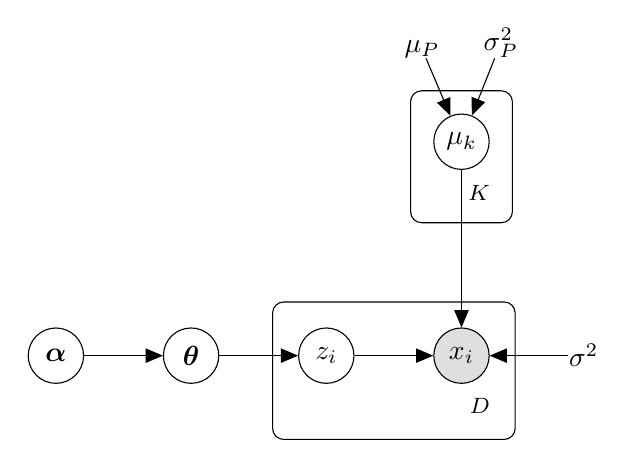
\begin{tikzpicture}
  % Nodes
  % parameters and data
	\node[obs]           (X)    {$x_i$}; %
	\node[latent, above = 2 of X]  (mu) {$\mu_k$};
	\node[const, above = 0.7 of mu, xshift=-0.5cm]     (muP)    {$\mu_P$}; %
	\node[const, above = 0.7 of mu, , xshift=0.5cm]  (sigmaP) {$\sigma^2_P$};
  \node[const, right= of X]  (sigma) {$\sigma^2$};
	\node[latent, left = of X]  (Z) {$z_i$};
	\node[latent, left = of Z]  (theta) {$\btheta$};
	\node[latent, left = of theta]  (alpha) {$\balpha$};
  % explanations of the nodes
%	\node[const, left = of x] (x_ex) {Covariates};
%	\node[const, left = of gamma] (gamma_ex) {Topic};
%	\node[const, left = of sigma] (sigma_ex) {Coefficients}; 
%	\node[const, above = of theta] (theta_ex) {Document-Topic\\ proprtions};
 % Edges
  \edge{mu}{X}; \edge{muP}{mu}; \edge{sigmaP}{mu};
  \edge{alpha}{theta}; \edge{theta}{Z}; \edge{Z}{X};
  \edge{sigma}{X};
 % Plates
	\plate[inner sep=9pt]{plate1}{
    (X)(Z)
  }{$D$};

	\plate[inner sep=8pt]{plate2}{
    (mu)
  }{$K$};
\end{tikzpicture}
\caption{Gaussian Mixture}
\end{figure}

\begin{align}
\mu_k &\sim \mathcal{N} (\mu_{\rm P}, \sigma^2_{\rm P}), \ \ k = 1, \cdots, K \\
\boldsymbol{\theta} &\sim {\rm Dir}(\boldsymbol{\alpha}), \  \ \ \boldsymbol{\alpha} = (\alpha_1, \cdots, \alpha_K) \\
z_i &\sim {\rm Multi}(1 | \boldsymbol{\theta}), \ \ i = 1, \cdots, D \\
x_i &\sim \mathcal{N} (u_{z_i = k}, \sigma^2), \ \ i = 1, \cdots, D
\end{align}

\section{Gibbs Sampling}
\subsection{全確率変数の結合分布}
\begin{align}
  &\quad\quad p(\bx, \btheta, \bz, \bmu | \balpha, \mu_P, \sigma^2_P, \sigma^2)\\
  &= p(\bx | \bz, \bmu, \sigma^2) p(\btheta, \bz, \bmu | \balpha, \mu_P, \sigma^2_P, \sigma^2)\\
  &= p(\bx | \bz, \bmu, \sigma^2) p(\bz|\btheta)p(\btheta|\balpha)p(\bmu|\mu_P, \sigma^2_P)\\[3pt]
  &= \prod_{i=1}^{D} \left\{ p(x_i | \mu_{z_i}, \sigma^2) p(z_i|\btheta) \right\} \cdot p(\btheta|\balpha) \cdot \prod_{k=1}^{K} p(\mu_k | \mu_P, \sigma_P^2)
\end{align}

\subsection{更新式}
\subsubsection{$\boldsymbol{z_i}$のサンプリング}
\begin{align}
  &\qquad p(z_i = k | x_i, \bx^\deli, \bz^\deli, \btheta, \bmu, \balpha, \mu_P, \sigma^2_P, \sigma^2)\\
  &\propto p(z_i=k, x_i, \bx^\deli, \bz^\deli, \btheta, \bmu | \balpha, \mu_P, \sigma^2_P, \sigma^2)\\
&= p(x_i|z_i=k, \bx^\deli, \bz^\deli, \btheta, \bmu, \balpha, \mu_P, \sigma^2_P, \sigma^2) \cdot p(z_i=k | \bx^\deli, \bz^\deli, \btheta, \bmu | \balpha, \mu_P, \sigma^2_P, \sigma^2)\\
  &= p(x_i| z_i=k, \mu_k, \sigma^2) \cdot p(z_i=k | \bx^\deli, \bz^\deli, \btheta, \bmu) \cdot p(\bx^\deli, \bz^\deli, \btheta, \bmu | \balpha, \mu_P, \sigma^2_P, \sigma^2)\\
  &= p(x_i | \mu_{z_i=k}, \sigma^2) \cdot p(z_i=k | \btheta) \cdot p(\bx^\deli, \bz^\deli, \btheta, \bmu | \balpha, \mu_P, \sigma^2_P, \sigma^2)\\
  &\propto \underbrace{p(x_i |  \mu_{z_i=k}, \sigma^2)}_{\rm Normal \ Distribution} \cdot \underbrace{ p(z_i=k | \btheta) }_{\theta_k}
\end{align}

\subsubsection{$\boldsymbol{\theta}$のサンプリング}
\begin{align}
  &\qquad p(\btheta | \bx, \bz, \bmu, \balpha, \mu_P, \sigma^2_P, \sigma^2)\\
  &\propto p(\btheta, \bx, \bz, \bmu | \balpha, \mu_P, \sigma^2_P, \sigma^2)\\
  &= p(\bx | \btheta, \bz, \bmu, \balpha, \mu_P, \sigma^2_P, \sigma^2) p(\btheta, \bz, \bmu | \balpha, \mu_P, \sigma^2_P, \sigma^2) \\
  &= p(\bx| \bz, \bmu, \sigma^2) p(\bz | \btheta) p(\btheta | \bmu, \balpha, \mu_P, \sigma^2_P, \sigma^2) p(\bmu | \balpha, \mu_P, \sigma^2_P, \sigma^2) \\[3pt]
  &\propto \underbrace{p(\bz | \btheta)}_{\rm Multi} \underbrace{p(\btheta | \balpha)}_{\rm Dir}\\
  &\propto \prod_{k=i}^{K} \theta_{k}^{n_k + \alpha_k -1}, \ \ {\rm where \ }  n_k = \sum_{i=1}^{D} \delta(z_i=k)
\end{align}
$\btheta$はDirichlet分布からなので正規化項も考えると、
\begin{align}
  \frac{\Gamma \left( \sum_{k=1}^K n_k + \alpha_k \right)}{\prod_{k=1}^K \Gamma(n_k + \alpha_k)} \prod_{k=1}^K \theta_{k}^{n_k + \alpha_k - 1}
\end{align}

\subsubsection{$\boldsymbol{\mu_k}$のサンプリング}
\begin{align}
  &\qquad p(\mu_k | \bmu^{\backslash k}, \bx, \bz, \btheta, \balpha, \mu_P, \sigma^2_P, \sigma^2) \\
  &\propto p(\mu_k, \bmu^{\backslash k}, \bx, \bz, \btheta | \balpha, \mu_P, \sigma^2_P, \sigma^2)\\
  &= p(\bx | \bmu, \bmu^{\backslash k}, \bz, \btheta, \balpha, \mu_P, \sigma_P^2, \sigma^2) p(\bmu, \bmu^{\backslash k} \bz, \btheta | \balpha, \mu_P, \sigma_P^2, \sigma^2)\\
  &= p(\bx | \bmu, \bmu^{\backslash k}, \bz, \sigma^2) p(\mu_k | \mu_P, \sigma^2_P) p(\bmu^{\backslash k}, \bz, \btheta | \balpha, \mu_P, \sigma_P^2, \sigma^2)\\
  &\propto \underbrace{p(\bx | \bmu, \bz, \sigma^2)}_{\rm Normal} \underbrace{ p(\mu_k | \mu_P, \sigma^2_P)}_{\rm Normal} \\
  &\propto \prod_{k=1}^{K} \left[ \left\{ \prod_{i=1}^{D} \frac{1}{\sqrt{\sigma^2}} \exp \left( - \frac{(x_i - \mu_k)^2}{2 \sigma^2} \right)  \cdot \delta(z_i = k) \right\} \times \left\{  \frac{1}{\sqrt{\sigma_P^2}} \exp \left(  - \frac{(\mu_k - \mu_P)^2}{2 \sigma_P^2} \right) \right\} \right]
\end{align}
\href{https://en.wikipedia.org/wiki/Conjugate_prior#Table_of_conjugate_distributions}{WikipediaのConjugate prior}の記事を参考にすると、更新後の平均は、
\begin{align}
  \left. \left( \frac{\mu_P}{\sigma_P^2} + \frac{\sum_{i=1}^{D} x_i \cdot \delta(z_i=k)}{\sigma^2} \right) \middle/ \left( \frac{1}{\sigma_P^2} + \frac{\sum_{i=1}^{D} \delta (z_i = k)}{\sigma^2} \right)   \right. , \ \ \ k=1, \cdots, K
\end{align}
分散は、
\begin{align}
  \left( \frac{1}{\sigma^2_P} + \frac{\sum_{i=1}^{D} \delta(z_i=k)}{\sigma^2} \right)^{-1} , \ \ \ k=1, \cdots, K
\end{align}
となる。

\section{Collapsed Gibbs Sampling}
$\btheta$と$\bmu$を積分消去する。このときのグラフィカルモデルは以下のようになる。
\begin{figure}[H]
\centering
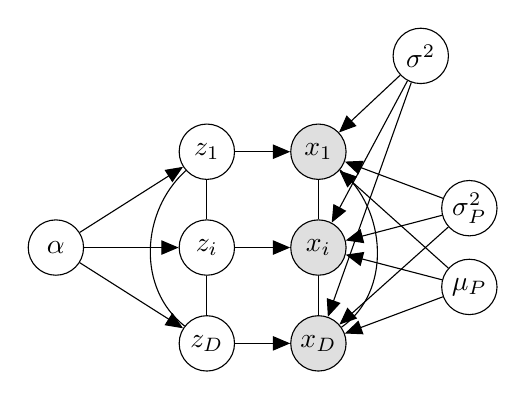
\begin{tikzpicture}
  % Nodes
  % parameters and data
	\node[obs]           (X1)    {$x_1$}; %
  \node[obs, below = 0.5 of X1]    (Xi)    {$x_i$};
  \node[obs, below = 0.5 of Xi]    (XD)    {$x_D$};
	\node[latent, left = 0.7 of X1]           (Z1)    {$z_1$}; %
  \node[latent, above = 0.5 of X1,  xshift=1.3cm] (sigma)    {$\sigma^2$};
  \node[latent, below = 0.5 of Z1]    (Zi)    {$z_i$};
  \node[latent, below = 0.5 of Zi]    (ZD)    {$z_D$};
  \node[latent, right = 1.2 of Xi, yshift=-0.5cm] (muP)    {$\mu_P$};
  \node[latent, right = 1.2 of Xi, yshift=0.5cm] (sigmaP)    {$\sigma^2_P$};
  \node[latent, left = 1.2 of Zi] (alpha)    {$\alpha$};
 % Draw
  \draw(X1)--(Xi);\draw(Xi)--(XD); \draw(Z1)--(Zi);\draw(Zi)--(ZD);
  \draw(X1) [out=320, in=35] to (XD);\draw(Z1) [out=222, in=142] to (ZD);
 % Edges
  \edge{Z1}{X1};\edge{Zi}{Xi};\edge{ZD}{XD};
  \edge{sigma}{X1};\edge{sigma}{Xi};\edge{sigma}{XD};
  \edge{muP}{X1};\edge{muP}{Xi};\edge{muP}{XD};
  \edge{sigmaP}{X1};\edge{sigmaP}{Xi};\edge{sigmaP}{XD};
  \edge{alpha}{Z1};\edge{alpha}{Zi};\edge{alpha}{ZD};
 % Plates
\end{tikzpicture}
\caption{Collapsed Gibbs Sampling}
\end{figure}
周辺化されることで、隠れ変数やデータに依存関係が生まれていることに注意する必要がある。依存関係があるため、$z$を全て同時にサンプリングすることはできないが、$z_1, \cdots, z_D$のように1つずつサンプリングすることは可能である。ある$z_i$は、それ以外のデータ$\bz^\deli$が与えられた状態でサンプリングする。



\begin{align}
  &\qquad p(z_i = k| x_i, \bx^\deli, \bz^\deli, \balpha, \mu_P, \sigma^2_P, \sigma^2)\\
  &\propto p(z_i=k, x_i, \bx^\deli, \bz^\deli | \balpha, \mu_P, \sigma^2_P, \sigma^2)\\
  &= p(x_i | z_i=k, \bx^\deli, \bz^\deli, \balpha, \mu_P, \sigma^2_P, \sigma^2) p(z_i=k, \bx^\deli, \bz^\deli | \balpha, \mu_P, \sigma^2_P, \sigma^2)\\
  &= p(x_i | z_i=k, \bx^\deli, \bz^\deli, \balpha, \mu_P, \sigma^2_P, \sigma^2) p(z_i=k | \bx^\deli, \bz^\deli, \balpha, \mu_P, \sigma^2_P, \sigma^2) p(\bx^\deli, \bz^\deli | \balpha, \mu_P, \sigma^2_P, \sigma^2)\\
  &\propto p(x_i | z_i=k, \bx^\deli, \bz^\deli, \balpha, \mu_P, \sigma^2_P, \sigma^2) p(z_i=k| \bx^\deli, \bz^\deli, \balpha, \mu_P, \sigma^2_P, \sigma^2)\\
  &= p(x_i | z_i=k, \bx^\deli, \bz^\deli,  \mu_P, \sigma^2_P, \sigma^2) p(z_i=k| \bx^\deli, \bz^\deli, \balpha)\\
  &= \int p(x_i| z_i=k, \bmu, \bx^\deli, \bz^\deli,  \mu_P, \sigma_P^2, \sigma^2) p(\bmu |z_i=k, \bx^\deli, \bz^\deli,  \mu_P, \sigma^2_P, \sigma^2) d\bmu \\
  &\qquad \qquad \qquad \qquad \qquad \qquad \qquad \qquad \qquad \times \int p(z_i=k| \btheta, \bx^\deli, \bz^\deli, \balpha) p(\btheta | \bx^\deli, \bz^\deli, \balpha) d\btheta\\
  &= \int p(x_i | z_i=k, \mu_k, \sigma^2) p(\mu_k | \bx^\deli, \bz^\deli, \mu_P, \sigma^2_P, \sigma^2) d\mu_k \int p(z_i =k|\btheta) p(\btheta | \bz^\deli,\balpha) d\btheta \label{pred1}\\[3.5pt]
  %&= \left[ \int \frac{1}{\sqrt{\sigma^2}} \exp \left\{ -\frac{(x_i - \mu_k)^2}{2 \sigma^2} \right\} \times \frac{1}{\sqrt{\sigma^2_P}} \exp \left\{ -\frac{(\mu_k - \mu_P)^2}{2 \sigma^2_P} \right\} d\mu_k \right] \cdot  \E_{p(\btheta | \bz^\deli,\balpha)} \left[ p(z_i | \btheta) \right] \\[4pt]
  \begin{split}
  &= \cN(x_i | \mu_{\rm New}, \sigma_{\rm New}) \cdot \frac{n_k^{\backslash i} + \alpha_k}{\sum_{k=1}^{K} n_k^{\backslash i} + \alpha_k},
\qquad {\rm where} \ \ 
    \begin{cases} 
      \left. \mu_{\rm New} = \left( \frac{\mu_P}{\sigma_P^2} + \frac{\mu_k}{\sigma^2} \right) \middle/ \left( \frac{1}{\sigma_P^2} + \frac{1}{\sigma^2} \right) \right.   \\[8pt] 
     \sigma_{\rm New} = \left( \frac{1}{\sigma_P^2} + \frac{1}{\sigma^2}  \right)^{-1}
    \end{cases} 
  \end{split}
  %&= \left\{ \left( \frac{\mu_P}{\sigma_P^2} + \frac{\sum_{d=1}^{D^{\backslash i}} x_d \cdot \delta(z_d=k)}{\sigma^2} \right) \middle/ \left( \frac{1}{\sigma_P^2} + \frac{\sum_{d=1}^{D^{\backslash i}} \delta (z_d = k)}{\sigma^2} \right)   \right\} \cdot \frac{n_k^{\backslash i} + \alpha_k}{\sum_{k=1}^{K} n_k^{\backslash i} + \alpha_k}
\end{align}

式(\ref{pred1})は、それぞれ$x_i$、$z_i$に関する予測分布 (posterior predictive distribution)\footnote{Wikipedia, Coonjugate Prior: https://en.wikipedia.org/wiki/Conjugate\_prior\#Table\_of\_conjugate\_distributions}であると解釈することができる。第1項はNormalとNormal、第2項はMultinomial (Categorical)とDirichletである。

\end{document}
